\documentclass[semifinal,survey]{cpecmu}

%% This is a sample document demonstrating how to use the CPECMU
%% project template. If you are having trouble, see "cpecmu.pdf" for
%% documentation.

\projectNo{S808-1}
\acadyear{2025}

\titleTH{ระบบตรวจจับภัยคุกคามในเทคโนโลยีปฏิบัติการ (OT) สำหรับโรงงานอุตสาหกรรม}
\titleEN{Anomaly Detection in Operational Technology for Industrial Control Systems}

\author{นายธนกฤต บุญยัง}{Tanakrit boonyoung}{650612084}
\author{นายศุภกร สุวรรณภพ}{Suppakorn suwannapop}{650612100}
\author{นายอดิศร สันเจริญ}{Adisorn sancharoen}{650612104}

\cpeadvisor{kampol}
\cpecommittee{kasemsit}
\committee{อ.นพรุจ\,ซื่อตรง}{Nopparuj\,Suetrong}

%% Some possible packages to include:
\usepackage[final]{graphicx} % for including graphics

%% Add bookmarks and hyperlinks in the document.
\PassOptionsToPackage{hyphens}{url}
\usepackage[colorlinks=true,allcolors=Blue4,citecolor=red,linktoc=all]{hyperref}
\def\UrlLeft#1\UrlRight{$#1$}

%% Needed just by this example, but maybe not by most reports
\usepackage{afterpage} % for outputting
\usepackage{pdflscape} % for landscape figures and tables. 
\usepackage{subcaption}
\usepackage{tabularx}
\usepackage{makecell}
\usepackage{float}
%% Some other useful packages. Look these up to find out how to use
%% them.
% \usepackage{natbib}    % for author-year citation styles
% \usepackage{txfonts}
% \usepackage{appendix}  % for appendices on a per-chapter basis
% \usepackage{xtab}      % for tables that go over multiple pages
% \usepackage{subfigure} % for subfigures within a figure
% \usepackage{pstricks,pdftricks} % for access to special PostScript and PDF commands
% \usepackage{nomencl}   % if you have a list of abbreviations

%% if you're having problems with overfull boxes, you may need to increase
%% the tolerance to 9999
% \tolerance=9999
\nocite{*}
\bibliographystyle{plain}
% \bibliographystyle{IEEEbib}

% \renewcommand{\topfraction}{0.85}
% \renewcommand{\textfraction}{0.1}
% \renewcommand{\floatpagefraction}{0.75}

%% Example for glossary entry
%% Need to use glossary option
%% See glossaries package for complete documentation.
\ifglossary
  \newglossaryentry{lorem ipsum}{
    name=lorem ipsum,
    description={derived from Latin dolorem ipsum, translated as ``pain itself''}
  }
\fi

%% Uncomment this command to preview only specified LaTeX file(s)
%% imported with \include command below.
%% Any other file imported via \include but not specified here will not
%% be previewed.
%% Useful if your report is large, as you might not want to build
%% the entire file when editing a certain part of your report.
% \includeonly{chapters/intro,chapters/background}

\begin{document}
\maketitle
\makesignature

\ifproject
\begin{abstractTH}
\hspace{2em} ในยุคอุตสาหกรรม 4.0 โรงงานจำนวนมากได้ปรับใช้ ระบบควบคุมอัตโนมัติ (Industrial Control Systems: ICS) ที่เชื่อมโยงกับ เทคโนโลยีปฏิบัติการ (Operational Technology: OT) เพื่อตรวจวัดและควบคุมกระบวนการผลิตแบบเรียลไทม์ อย่างไรก็ตาม ความเชื่อมโยงดังกล่าวก่อให้เกิดความเสี่ยงจากภัยคุกคามทางไซเบอร์ ซึ่งอาจสร้างผลกระทบต่อ เศรษฐกิจ ความปลอดภัยของบุคลากร และสิ่งแวดล้อม

โครงงานนี้มีวัตถุประสงค์เพื่อพัฒนา ต้นแบบระบบตรวจจับความผิดปกติ (Anomaly/Intrusion Detection System) โดยใช้เทคนิค การเรียนรู้เชิงลึก (Deep Learning) ที่มุ่งเน้นการวิเคราะห์ ข้อมูลลำดับเวลา (time-series data) ของเซนเซอร์และแอกชูเอเตอร์ในระบบ OT

กระบวนการดำเนินงานประกอบด้วย การจัดเตรียมและทำความสะอาดข้อมูล (Preprocessing), การออกแบบคุณลักษณะ (Feature Engineering), การสร้างหน้าต่างเวลา (Sliding Window) และการ \\ พัฒนาโมเดลตรวจจับความผิดปกติ โดยใช้สถาปัตยกรรม 1D CNN-LSTM ซึ่งสามารถเรียนรู้ได้ทั้ง ความสัมพันธ์เชิงเวลา (temporal dependencies) และ ความสัมพันธ์เชิงลักษณะ (spatial/feature dependencies) ของข้อมูลเซนเซอร์

ผลลัพธ์ของโมเดลถูกประเมินด้วยตัวชี้วัดมาตรฐาน ได้แก่ Accuracy, Precision, Recall, F1-score รวมถึงการวิเคราะห์เชิงลึกเพื่อยืนยันความสามารถของโมเดลในการจำแนก เหตุการณ์ปกติ และ เหตุการณ์โจมตี (Anomaly events) ได้อย่างมีประสิทธิภาพ

\end{abstractTH}

\begin{abstract}
\hspace{2em} In the era of Industry 4.0, many factories have adopted Industrial Control Systems (ICS) integrated with Operational Technology (OT) to monitor and control production processes in real time. However, this interconnection introduces potential cybersecurity risks, which may significantly impact the economy, personnel safety, and the environment.

This project aims to develop a prototype anomaly/intrusion detection system using Deep Learning techniques, focusing on the analysis of time-series data obtained from sensors and actuators within OT systems.

The research methodology includes data preprocessing, feature engineering, sliding window generation, and the design of an anomaly detection model based on the 1D CNN-LSTM architecture. This hybrid approach enables the model to capture both temporal dependencies and feature-level (spatial) correlations within sensor data.

The performance of the proposed model is evaluated using standard metrics such as Accuracy, Precision, Recall, and F1-score, along with further analysis to verify its capability in effectively distinguishing between normal operations and attack/anomaly events. The outcome of this study contributes to enhancing the cyber resilience of ICS/OT systems and provides a foundation for practical applications in industrial cybersecurity.

\end{abstract}

\iffalse
\begin{dedication}
This document is dedicated to all Chiang Mai University students.

Dedication page is optional.
\end{dedication}
\fi % \iffalse

%\begin{acknowledgments}
%Your acknowledgments go here. Make sure it sits inside the
%\texttt{acknowledgment} environment.

%\acksign{2020}{5}{25}
%\end{acknowledgments}%
\fi % \ifproject

\contentspage

\ifproject
\figurelistpage

\tablelistpage
\fi % \ifproject

% \abbrlist % this page is optional

% \symlist % this page is optional

% \preface % this section is optional


\pagestyle{empty}\cleardoublepage
\normalspacing \setcounter{page}{1} \pagenumbering{arabic} \pagestyle{cpecmu}

\chapter{\ifenglish Introduction\else บทนำ\fi}

\section{\ifenglish Project rationale\else ที่มาของโครงงาน\fi}
ในปัจจุบันโรงงานอุตสาหกรรมจำนวนมากได้ยกระดับกระบวนการผลิตให้มีความเป็นอัตโนมัติสูงขึ้น โดยอาศัยระบบควบคุมอุตสาหกรรม (Industrial Control Systems: ICS) ที่ทำงานร่วมกับระบบเทคโนโลยีปฏิบัติการ (Operational Technology: OT) ซึ่งเชื่อมโยงเซนเซอร์และแอกชูเอเตอร์เข้ากับเครื่องจักรจริง อย่างไรก็ตาม การที่ระบบ OT ถูกเชื่อมต่อเข้ากับเครือข่ายดิจิทัลมากขึ้น ย่อมทำให้ความเสี่ยงจากภัยคุกคามทางไซเบอร์เพิ่มสูงขึ้นตามไปด้วย การโจมตีดังกล่าวอาจทำให้ข้อมูลสูญหายหรือบิดเบือน รวมถึงก่อให้เกิดความเสียหายต่อเครื่องจักร กระบวนการผลิต และความปลอดภัยของบุคลากรได้โดยตรง ดังนั้นโครงงานนี้จึงถูกริเริ่มขึ้นเพื่อพัฒนากลไกการตรวจจับพฤติกรรมที่ผิดปกติในระบบ OT โดยใช้เทคนิคการเรียนรู้ของเครื่อง (Machine Learning) เพื่อเสริมสร้างความปลอดภัยและลดความเสียหายที่อาจเกิดขึ้นในโรงงานอุตสาหกรรม

\section{\ifenglish Objectives\else วัตถุประสงค์ของโครงงาน\fi}
\begin{enumerate}
    \item ออกแบบและพัฒนาโมเดลตรวจจับความผิดปกติจากข้อมูลเซนเซอร์และแอกชูเอเตอร์ในระบบ OT โดยใช้การวิเคราะห์เชิงเวลา (time-series analysis) ร่วมกับโมเดลเชิงลึก เช่น CNN และ LSTM
    \item ระบุเหตุการณ์ที่มีลักษณะเป็นการโจมตีทางไซเบอร์หรือพฤติกรรมที่ผิดปกติในกระบวนการผลิต
    \item พัฒนาต้นแบบ (prototype) ที่สามารถนำไปประยุกต์ใช้กับสภาพแวดล้อมในโรงงานจริงได้
\end{enumerate}

\section{\ifenglish Project scope\else ขอบเขตของโครงงาน\fi}

\subsection{\ifenglish Hardware scope\else ขอบเขตด้านฮาร์ดแวร์\fi}
\begin{enumerate}
    \item โครงงานนี้ ไม่ได้มุ่งเน้นการพัฒนาหรือใช้งานฮาร์ดแวร์จริง เช่น PLC, ปั๊ม, หรือวาล์ว
    \item ส่วนประกอบเหล่านี้ถูก จำลองผ่านข้อมูลจาก SWaT dataset เท่านั้น
    \item การดำเนินงานทั้งหมดจึงมุ่งเน้นที่การวิเคราะห์เชิงข้อมูลและการออกแบบโมเดล Machine Learning โดยไม่เกี่ยวข้องกับการสร้างหรือทดสอบระบบฮาร์ดแวร์จริง
\end{enumerate}

\subsection{\ifenglish Software scope\else ขอบเขตด้านซอฟต์แวร์\fi}

\subsubsection{การเก็บและใช้ข้อมูล (Data Collection)}
\begin{enumerate}
    \item ใช้ชุดข้อมูล SWaT Dataset (Secure Water Treatment) ซึ่งเป็นข้อมูลจากระบบจำลองโรงงานน้ำประปาที่ใช้กันอย่างแพร่หลายในการศึกษาด้านความปลอดภัยของระบบ ICS/OT
    \item ข้อมูลประกอบด้วยค่าการทำงานของเซนเซอร์และแอกชูเอเตอร์ที่มีทั้งสภาวะปกติและสภาวะที่ถูกโจมตี
    \item การนำเข้าข้อมูลจะใช้วิธีการอ่านไฟล์ CSV และเตรียมข้อมูลให้อยู่ในรูปแบบที่เหมาะสมต่อการประมวลผล
\end{enumerate}

\subsubsection{การตรวจจับและจำแนกความผิดปกติ (Threat Detection and Classification) }
\begin{enumerate}
    \item มุ่งเน้นการตรวจจับเหตุการณ์ที่มีลักษณะผิดปกติ เช่น การเปลี่ยนค่าของเซนเซอร์อย่างผิดธรรมชาติ หรือการสั่งการอุปกรณ์ที่ไม่สอดคล้องกับกระบวนการจริง
    \item การจำแนกความผิดปกติออกเป็นสองกลุ่มหลัก ได้แก่
    \begin{enumerate}
        \item เหตุการณ์ปกติ (Normal events)
        \item เหตุการณ์โจมตี/ผิดปกติ (Anomaly/Attack events)
    \end{enumerate}
    \item การสร้าง Label จะอ้างอิงจากช่วงเวลาที่กำหนดไว้ในเอกสาร SWaT dataset
\end{enumerate}

\subsubsection{การประมวลผลและจัดการข้อมูล (Data Implementation)}
\begin{enumerate}
    \item การทำความสะอาดข้อมูล (data preprocessing) เช่น การจัดการค่าที่หายไป, การแทนค่าผิดปกติ, และการ normalize ข้อมูลให้อยู่ในสเกลเดียวกัน
    \item การแบ่งข้อมูลออกเป็น Training set, Validation set และ Test set โดยอ้างอิงตามลำดับเวลาเพื่อเลี่ยงการรั่วไหลของข้อมูล (data leakage)
    \item การสร้าง sliding windows สำหรับข้อมูลเชิงเวลา (time-series) เพื่อเตรียมให้เป็นอินพุตของโมเดล
\end{enumerate}

\subsubsection{การสร้างโมเดลและเปรียบเทียบประสิทธิภาพ (Model Comparison and Performance Evaluation)}
\begin{enumerate}
    \item พัฒนาโมเดลตรวจจับความผิดปกติที่อิงกับ Deep Learning ได้แก่ 
    \begin{enumerate}
        \item Convolutional Neural Network (CNN)
        \item  Long Short-Term Memory (LSTM)
    \end{enumerate}
    \item ทดสอบโมเดลหลายรูปแบบ เช่น CNN 1D สำหรับจับ pattern ตามลำดับเวลา และ LSTM สำหรับตรวจจับ dependency ระหว่างข้อมูลในช่วงยาว
    \item ประเมินผลลัพธ์ด้วยตัวชี้วัดมาตรฐาน
    \begin{enumerate}
        \item Accuracy, Precision
        \item Recall, F1-score
        \item Confusion Matrix 
        \item AUC-PR/ROC
    \end{enumerate}
    \item เปรียบเทียบประสิทธิภาพของแต่ละโมเดลเพื่อหาวิธีที่เหมาะสมที่สุดต่อการใช้งาน
\end{enumerate}

\subsubsection{ผลลัพธ์ที่คาดว่าจะได้รับ (Expected Outcomes)}
\begin{enumerate}
    \item ได้ต้นแบบ (Prototype) ของระบบตรวจจับความผิดปกติในข้อมูลจากระบบ ICS/OT
    \item โมเดลที่พัฒนาแล้วสามารถแยกความแตกต่างระหว่างเหตุการณ์ปกติและเหตุการณ์ผิดปกติได้ในระดับที่แม่นยำ
    \item ได้ชุดข้อมูลและโค้ดที่สามารถนำไปปรับใช้หรือต่อยอดในงานวิจัยด้านความปลอดภัยไซเบอร์สำหรับระบบอุตสาหกรรม
    \item สนับสนุนการเพิ่มมาตรการด้าน ความมั่นคงปลอดภัยเชิงปฏิบัติการ (Operational Security) ในโรงงานอุตสาหกรรม
\end{enumerate}

\section{\ifenglish Expected outcomes\else ประโยชน์ที่ได้รับ\fi}

\subsubsection{ด้านความรู้และความเข้าใจ}
\begin{enumerate}
    \item ได้ความเข้าใจเชิงลึกเกี่ยวกับประเด็นด้านความมั่นคงปลอดภัยในระบบควบคุมอุตสาหกรรม (OT/ICS)
    \item เพิ่มพูนทักษะในการนำ Machine Learning มาประยุกต์ใช้กับข้อมูลเชิงเวลา (time-series)
\end{enumerate}

\subsubsection{ด้านการพัฒนาเทคโนโลยี}
\begin{enumerate}
    \item ได้ต้นแบบ (Prototype) ของระบบตรวจจับความผิดปกติที่สามารถนำไปต่อยอดการพัฒนาระบบจริงได้
    \item แสดงให้เห็นความเป็นไปได้ของการนำ AI/ML มาใช้แก้ปัญหาความปลอดภัยในภาคอุตสาหกรรม
\end{enumerate}

\subsubsection{ด้านการประยุกต์ใช้}
\begin{enumerate}
    \item ผลงานที่ได้สามารถนำไปใช้ตรวจจับการโจมตีหรือพฤติกรรมผิดปกติในโรงงานอุตสาหกรรมจริง
    \item ช่วยเพิ่มความปลอดภัยทั้งในด้านข้อมูล เครื่องจักร และบุคลากร ลดความเสี่ยงจากการหยุดชะงักของกระบวนการผลิต
\end{enumerate}

\subsubsection{ด้านการวิจัยและการศึกษา}
\begin{enumerate}
    \item สามารถนำองค์ความรู้และผลลัพธ์ไปต่อยอดในเชิงวิจัยด้านความปลอดภัยไซเบอร์สำหรับระบบอุตสาหกรรม
    \item เป็นกรณีศึกษาในการบูรณาการ Machine Learning กับความปลอดภัยไซเบอร์ (AI for Cybersecurity)
\end{enumerate}

\section{\ifenglish Technology and tools\else เทคโนโลยีและเครื่องมือที่ใช้\fi}

\subsection{\ifenglish Hardware technology\else เทคโนโลยีด้านฮาร์ดแวร์\fi}

\subsection{\ifenglish Software technology\else เทคโนโลยีด้านซอฟต์แวร์\fi}

\section{\ifenglish Project plan\else แผนการดำเนินงาน\fi}

\begin{plan}{6}{2020}{2}{2021}
    \planitem{7}{2020}{8}{2020}{ศึกษาค้นคว้า}
    \planitem{8}{2020}{1}{2021}{ชิล}
    \planitem{2}{2021}{2}{2021}{เผา}
    \planitem{12}{2019}{1}{2022}{ทดสอบ}
\end{plan}

\section{\ifenglish Roles and responsibilities\else บทบาทและความรับผิดชอบ\fi}
อธิบายว่าในการทำงาน นศ. มีการกำหนดบทบาทและแบ่งหน้าที่งานอย่างไรในการทำงาน จำเป็นต้องใช้ความรู้ใดในการทำงานบ้าง

\section{\ifenglish%
Impacts of this project on society, health, safety, legal, and cultural issues
\else%
ผลกระทบด้านสังคม สุขภาพ ความปลอดภัย กฎหมาย และวัฒนธรรม
\fi}

แนวทางและโยชน์ในการประยุกต์ใช้งานโครงงานกับงานในด้านอื่นๆ รวมถึงผลกระทบในด้านสังคมและสิ่งแวดล้อมจากการใช้ความรู้ทางวิศวกรรมที่ได้

\chapter{\ifenglish Background Knowledge and Theory\else ทฤษฎีที่เกี่ยวข้อง\fi}

การทำโครงงาน เริ่มต้นด้วยการศึกษาค้นคว้า ทฤษฎีที่เกี่ยวข้อง หรือ งานวิจัย/โครงงาน ที่เคยมีผู้นำเสนอไว้แล้ว ซึ่งเนื้อหาในบทนี้ก็จะเกี่ยวกับการอธิบายถึงสิ่งที่เกี่ยวข้องกับโครงงาน เพื่อให้ผู้อ่านเข้าใจเนื้อหาในบทถัดๆ ไปได้ง่ายขึ้น

\section{Operational Technology (OT) และ Industrial Control Systems (ICS)}

\hspace{2em} Operational Technology (OT) คือเทคโนโลยีที่ใช้สำหรับตรวจสอบและควบคุมกระบวนการทางกายภาพในโรงงานอุตสาหกรรมหรือโครงสร้างพื้นฐานที่สำคัญ เช่น ระบบไฟฟ้า ระบบน้ำมัน และระบบบำบัดน้ำเสีย จุดเด่นของ OT คือการทำงานที่ต้องเน้น ความต่อเนื่อง ความเสถียร และความปลอดภัย มากกว่า IT (Information Technology) ที่มุ่งเน้นการประมวลผลข้อมูลและธุรกรรมเป็นหลัก

\subsubsection*{Industrial Control Systems (ICS) เป็นกลุ่มของระบบที่ใช้ควบคุมและจัดการการทำงานของ OT โดยมีตัวอย่างที่สำคัญ ได้แก่}
\begin{enumerate}
  \item Supervisory Control and Data Acquisition (SCADA) ใช้สำหรับควบคุมและตรวจสอบระบบขนาดใหญ่ที่กระจายตัว
  \item Distributed Control System (DCS) ใช้ควบคุมกระบวนการแบบต่อเนื่อง เช่น โรงกลั่นน้ำมัน
  \item Programmable Logic Controller (PLC) ใช้ในกระบวนการที่ต้องการการควบคุมแบบเฉพาะกิจ
\end{enumerate}

\section{ความมั่นคงปลอดภัยไซเบอร์ในระบบ OT/ICS}

\hspace{2em} ระบบ ICS เดิมถูกออกแบบมาเพื่อเน้นความทนทานและการทำงานอย่างต่อเนื่อง โดยไม่ได้คำนึงถึงการป้องกันภัยไซเบอร์ ทำให้มีช่องโหว่ต่อการโจมตี เช่น:
\begin{enumerate}
  \item Stuxnet (2010): มัลแวร์ที่แทรกแซงการทำงานของ PLC ในโรงงานนิวเคลียร์อิหร่าน
  \item Ukraine Power Grid Attack (2015): การโจมตีระบบไฟฟ้าทำให้เกิดการดับไฟในวงกว้าง
\end{enumerate}
\indent
กรณีศึกษาดังกล่าวสะท้อนว่าภัยคุกคามไซเบอร์สามารถสร้างความเสียหายทั้งด้านเศรษฐกิจ ความมั่นคง และความปลอดภัยของประชาชน การพัฒนา ระบบตรวจจับความผิดปกติ (Anomaly Detection) จึงมีความสำคัญอย่างยิ่งใน OT

\subsection{Anomaly Detection}
\hspace{2em} Anomaly Detection คือกระบวนการระบุข้อมูลที่เบี่ยงเบนไปจากรูปแบบปกติ ซึ่งอาจเกิดจากการโจมตี ความผิดพลาดของอุปกรณ์ หรือความผิดปกติของกระบวนการ โดยทั่วไปแบ่งได้เป็น 3 ประเภท:

\begin{enumerate}
  \item Point Anomaly: ข้อมูลจุดเดียวที่ผิดปกติ (เช่น ค่า Sensor พุ่งสูงกว่าปกติ)
  \item Contextual Anomaly: ข้อมูลที่ปกติในบางบริบท แต่ผิดปกติในอีกบริบทหนึ่ง (เช่น ค่าน้ำสูงในฤดูฝนเป็นเรื่องปกติ แต่สูงในฤดูแล้งถือว่าผิดปกติ)
  \item Collective Anomaly: ลำดับข้อมูลหลายจุดที่รวมกันแล้วผิดปกติ (เช่น การทำงานของ Pump และ Valve ที่ไม่สัมพันธ์กัน)
\end{enumerate}
\indent
สำหรับระบบ ICS Collective Anomaly มีความสำคัญมาก เนื่องจากข้อมูลจาก Sensor และ Actuator อยู่ในรูปแบบ Time-Series ที่ต้องพิจารณาลำดับเวลา

\section{ Secure Water Treatment (SWaT) Dataset}
\hspace{2em} Secure Water Treatment (SWaT) Dataset เป็นชุดข้อมูลที่สร้างขึ้นจากโรงงานจำลองระบบบำบัดน้ำ (Water Treatment Testbed) โดย iTrust Lab, Singapore University of Technology and Design (SUTD) มีวัตถุประสงค์เพื่อใช้เป็น มาตรฐานกลาง (benchmark) สำหรับการวิจัยด้านความปลอดภัยไซเบอร์ในระบบควบคุมอุตสาหกรรม (ICS/SCADA)

\subsubsection{โครงสร้างของระบบ SWaT}
โรงงานจำลอง SWaT ออกแบบให้มีลักษณะใกล้เคียงโรงงานจริง โดยแบ่งออกเป็น 6 กระบวนการย่อย (Processes/Stages):

\begin{enumerate}
  \item P1: Raw Water Supply – ระบบสูบน้ำดิบเข้าสู่ถังเก็บ
  \item P2: Pre-treatment – การกรองเบื้องต้น (Ultrafiltration)
  \item P3: Chemical Dosing – การเติมสารเคมี เช่น กรด-ด่าง เพื่อปรับค่า pH
  \item P4: Membrane-based Ultra-Filtration – การกรองละเอียดด้วยเมมเบรน
  \item P5: Dechlorination – การกำจัดคลอรีนที่เหลืออยู่
  \item P6: Backwash and Product Storage – การล้างย้อนและการเก็บน้ำสะอาดในถังเก็บสุดท้าย
\end{enumerate}
\indent
ในแต่ละกระบวนการจะมีการติดตั้ง เซนเซอร์ (sensors) และ แอกชูเอเตอร์ (actuators) เช่น ปั๊ม (pumps), วาล์ว (valves), และเครื่องวัดระดับน้ำ (level sensors) ซึ่งควบคุมด้วย PLC (Programmable Logic Controllers) และเฝ้าติดตามผ่านระบบ SCADA

\subsubsection{ประเภทตัวแปรใน Dataset}
\hspace{2em} ข้อมูลที่บันทึกจาก SWaT เป็น Time-Series รายวินาที (1 sample/second) ครอบคลุมช่วงเวลา 11 วัน รวม 946,722 records และ 51 attributes

\subsubsection{ข้อมูลทางกายภาพ (Physical Properties)}
\begin{enumerate}
  \item Sensors (ตัวแปรต่อเนื่อง)
  \begin{enumerate}
    \item Flow (อัตราการไหล)
    \item Level (ระดับน้ำ)
    \item Pressure (ความดัน)
    \item Conductivity (ค่าการนำไฟฟ้า)
    \item pH (กรด-ด่าง)
    \item ORP (Oxidation-Reduction Potential)
    \item Temperature (อุณหภูมิ)
  \end{enumerate}
  \item Actuators (ตัวแปรไม่ต่อเนื่อง)
  \begin{enumerate}
    \item ปั๊ม (Pumps – เปิด/ปิด)
    \item วาล์ว (Motorized Valves – เปิด/ปิด)
    \item Dosing Pumps (สำหรับจ่ายสารเคมี)
  \end{enumerate}
\end{enumerate}

\subsubsection{สถานการณ์การโจมตี (Attack Scenarios)}
\hspace{2em} ในการทดลอง มีการออกแบบการโจมตีทั้งหมด 36 รูปแบบ แบ่งเป็น:

\begin{enumerate}
  \item Single Stage Single Point (SSSP) – โจมตีจุดเดียวในกระบวนการเดียว (26 ครั้ง)
  \item Single Stage Multi Point (SSMP) – โจมตีหลายจุดในกระบวนการเดียว (4 ครั้ง)
  \item Multi Stage Single Point (MSSP) – โจมตี 1 จุด แต่มีผลกระทบหลายกระบวนการ (2 ครั้ง)
  \item Multi Stage Multi Point (MSMP) – โจมตีหลายจุดในหลายกระบวนการ (4 ครั้ง)
\end{enumerate}

\subsubsection*{ตัวอย่าง:}
\begin{enumerate}
  \item ปลอมค่าจาก LIT101 (Level Sensor) ทำให้ระบบเข้าใจผิดว่าน้ำเต็มถัง และสั่งหยุดปั๊ม ส่งผลให้น้ำล้น (Overflow)
  \item ปลอมค่าจาก LIT301 ให้แสดงค่าสูงผิดปกติ ส่งผลให้ปั๊มทำงานต่อแม้น้ำหมด และเกิด Underflow และอาจทำให้ปั๊มเสียหาย
\end{enumerate}

\section{Machine Learning}
\hspace{2em} Machine Learning (ML) เป็นแขนงหนึ่งของปัญญาประดิษฐ์ (Artificial Intelligence: AI) ที่ช่วยให้ระบบสามารถเรียนรู้และปรับปรุงประสิทธิภาพจากข้อมูล โดยไม่ต้องเขียนกฎแบบตายตัวล่วงหน้า การป้อนข้อมูลจำนวนมากที่หลากหลายช่วยให้โมเดลสามารถสกัดรูปแบบ (patterns) และปรับปรุงความ \\ แม่นยำได้อย่างต่อเนื่อง

สำหรับโครงการนี้ ML ถูกนำมาใช้ในการตรวจจับความผิดปกติ (Anomaly Detection) ใน ข้อมูลเชิงเวลา (time-series) ที่ได้จาก ระบบควบคุมอุตสาหกรรม (ICS/OT) ซึ่งประกอบด้วยเซนเซอร์และแอกชูเอเตอร์ในระบบบำบัดน้ำ (SWaT dataset)

\section{Convolutional Neural Network – Long Short-Term Memory (CNN-LSTM)}
\hspace{2em} การตรวจจับความผิดปกติในข้อมูลเชิงเวลา (time-series anomaly detection) จำเป็นต้องอาศัยโมเดลที่สามารถสกัดคุณลักษณะเชิงลึกและในขณะเดียวกันต้องเข้าใจความสัมพันธ์เชิงลำดับเวลา โมเดล \\ CNN-LSTM จึงถูกนำมาใช้เพราะผสานข้อดีของ Convolutional Neural Network (CNN) และ Long Short-Term Memory (LSTM) เข้าด้วยกัน ทำให้สามารถจัดการกับข้อมูลจากระบบควบคุมอุตสาหกรรม (ICS) ที่มีความซับซ้อนสูงได้อย่างมีประสิทธิภาพ โดยเฉพาะข้อมูลจาก SWaT dataset ซึ่งประกอบด้วยข้อมูลจาก sensor และ actuator ที่บันทึกเป็นลำดับเวลา

\subsection{Convolutional Neural Network (CNN)}
\hspace{2em} CNN เป็นโครงข่ายประสาทเทียมที่พัฒนาขึ้นเพื่อตรวจจับและสกัดคุณลักษณะสำคัญจากข้อมูล โดยอาศัยการทำงานของ convolution filters ที่เลื่อนผ่านข้อมูลเพื่อค้นหารูปแบบซ้ำหรือความเปลี่ยนแปลงที่มีนัยสำคัญ ในบริบทของข้อมูลเชิงเวลา CNN สามารถทำหน้าที่ตรวจสอบการเปลี่ยนแปลงของค่า sensor ในช่วงสั้น ๆ ได้อย่างมีประสิทธิภาพ เช่น การแกว่งของระดับน้ำหรือการเปลี่ยนแปลงค่าความดันอย่างเฉียบพลัน นอกจากนี้ CNN ยังช่วยลดสัญญาณรบกวน (noise) และเน้นคุณลักษณะที่บ่งบอกถึงความผิดปกติได้อย่างชัดเจน

\subsection{Long Short-Term Memory (LSTM)}
\hspace{2em} LSTM เป็นโครงข่ายประสาทเทียมแบบ Recurrent Neural Network (RNN) ที่ถูกออกแบบมาเพื่อแก้ไขข้อจำกัดด้านการจำข้อมูลระยะยาวของ RNN ทั่วไป โดยใช้โครงสร้างที่มีกลไกสำคัญคือ forget gate, input gate และ output gate เพื่อกำหนดว่าข้อมูลใดควรถูกเก็บรักษาไว้และข้อมูลใดควรถูกลืมไป ทำให้ LSTM สามารถเรียนรู้ความสัมพันธ์ที่ซับซ้อนและยาวนานของข้อมูลเชิงเวลาได้อย่างมีประสิทธิภาพ สำหรับข้อมูลจาก SWaT dataset LSTM สามารถตรวจสอบความเชื่อมโยงของ sensor และ actuator ที่ทำงานต่อเนื่องหลายขั้นตอน เช่น ลำดับการเปิดปิดของปั๊มและวาล์ว ซึ่งอาจเป็นปัจจัยสำคัญที่ทำให้เกิดความผิดปกติในกระบวนการ

\subsection{CNN-LSTM for Anomaly Detection}
\hspace{2em} การผสมผสาน CNN และ LSTM เข้าไว้ด้วยกันในโมเดล CNN-LSTM ทำให้สามารถใช้ CNN ในการสกัดคุณลักษณะสำคัญจากข้อมูลเชิงเวลาในช่วงสั้น แล้วส่งผลลัพธ์ต่อให้ LSTM เพื่อเรียนรู้ความสัมพันธ์ที่ต่อเนื่องในระยะยาว แนวทางนี้ช่วยให้โมเดลสามารถจับพฤติกรรมผิดปกติที่ซับซ้อนในระบบ ICS ได้ดียิ่งขึ้น เมื่อเปรียบเทียบกับการใช้ CNN หรือ LSTM เพียงอย่างเดียว งานวิจัยจำนวนมากยืนยันว่าโมเดล CNN-LSTM มีประสิทธิภาพในการลดอัตราการตรวจจับผิดพลาด (false positives) และเพิ่มความแม่นยำในการตรวจจับ anomaly ได้ โดยเฉพาะอย่างยิ่งเมื่อใช้กับข้อมูลที่มีลักษณะ time-series แบบหลายตัวแปร (multivariate time-series) เช่นใน SWaT dataset

\subsection{Dense Layer และ Fully Connected Layer}
\hspace{2em} หลังจากที่ CNN และ LSTM ทำหน้าที่สกัดคุณลักษณะและจับความสัมพันธ์เชิงเวลาแล้ว ผลลัพธ์ที่ได้จะถูกส่งต่อไปยัง Dense Layer หรือ Fully Connected Layer เพื่อทำการรวมข้อมูลและสร้างการตัดสินใจสุดท้าย Dense Layer ทำงานโดยเชื่อมต่อทุกนิวรอนกับนิวรอนในชั้นถัดไป ช่วยให้โมเดลสามารถเรียนรู้การรวมคุณลักษณะที่ซับซ้อนและสร้างการจำแนก (classification) ระหว่างเหตุการณ์ปกติและเหตุการณ์ผิดปกติได้อย่างมีประสิทธิภาพ
ในโครงการนี้ Dense Layer ทำหน้าที่แปลง representation ที่ได้จาก CNN-LSTM ให้กลายเป็นค่าความน่าจะเป็น (probability) ของ class เช่น Normal (0) และ Anomaly (1)

\subsection{Activation Functions}
\hspace{2em} ฟังก์ชันกระตุ้น (Activation Functions) เป็นองค์ประกอบสำคัญของ Dense Layer ซึ่งใช้ในการกำหนดเส้นแบ่งเชิงเส้นหรือไม่เชิงเส้น เช่น:
\begin{enumerate}
  \item ReLU (Rectified Linear Unit): ใช้ในชั้นซ่อน (hidden layers) ของ CNN และ LSTM เพื่อลดปัญหา vanishing gradient และเร่งการเรียนรู้
  \item Sigmoid: เหมาะกับการจำแนกแบบ binary anomaly detection เนื่องจากผลลัพธ์อยู่ระหว่าง 0–1
  \item Softmax: ใช้สำหรับ multi-class anomaly detection เมื่อมีความผิดปกติหลายประเภท
\end{enumerate}

\subsection{Regularization Layers (Dropout และ Batch Normalization)}
\hspace{2em} เพื่อป้องกันการเกิด overfitting จากข้อมูลที่มีความซับซ้อนสูง เช่น SWaT dataset การเพิ่ม Regularization Layers มีความสำคัญมาก ได้แก่:
\begin{enumerate}
  \item Dropout Layer: ทำการสุ่มปิดบางนิวรอนระหว่างการฝึก เพื่อป้องกันไม่ให้โมเดลจดจำข้อมูลมากเกินไป แต่ช่วยให้เกิดการเรียนรู้ที่ครอบคลุมมากขึ้น
  \item Batch Normalization: ช่วยปรับค่าการกระจายของข้อมูลในแต่ละชั้นให้อยู่ในช่วงที่เหมาะสม ทำให้การฝึกโมเดลเสถียรและรวดเร็วขึ้น
\end{enumerate}

\section{Correlation Matrix}
\hspace{2em} Correlation Matrix เป็นเครื่องมือเชิงสถิติที่ใช้วิเคราะห์ความสัมพันธ์ระหว่างตัวแปรหลายตัวพร้อมกัน โดยจะแสดงค่า Correlation Coefficient ที่มีค่าตั้งแต่ -1 ถึง 1
\begin{enumerate}
  \item ค่า 1 หมายถึงความสัมพันธ์เชิงบวกอย่างสมบูรณ์ (เมื่อค่าของตัวแปรหนึ่งเพิ่ม อีกตัวก็เพิ่มตาม)
  \item ค่า -1 หมายถึงความสัมพันธ์เชิงลบอย่างสมบูรณ์ (เมื่อค่าของตัวแปรหนึ่งเพิ่ม อีกตัวจะลดลง)
  \item ค่า 0 หมายถึงไม่มีความสัมพันธ์
\end{enumerate}
สำหรับ SWaT dataset การสร้าง Correlation Matrix มีความสำคัญในหลายประเด็น ได้แก่
\begin{enumerate}
  \item การทำความเข้าใจความสัมพันธ์ของ Sensor และ Actuator: เช่น ระดับน้ำ (Level) ควรมีความสัมพันธ์กับการทำงานของปั๊ม (Pump) และวาล์ว (Valve)
  \item การตรวจหาความผิดปกติ (Anomaly): หาก correlation ระหว่าง sensor และ actuator ไม่เป็นไปตามปกติ เช่น ค่า Flow ไม่สัมพันธ์กับการเปิดปิด Valve อาจบ่งชี้ถึงการโจมตีหรือความผิดปกติในกระบวนการ
  \item Feature Selection: การวิเคราะห์ความสัมพันธ์ช่วยคัดเลือกตัวแปรที่สำคัญ และลด \\ multicollinearity เพื่อลด noise ก่อนนำเข้าสู่โมเดล Machine Learning
\end{enumerate}
\indent
การใช้ Correlation Matrix จึงเป็นขั้นตอนสำคัญใน Exploratory Data Analysis (EDA) ของโครงการนี้ เพื่อทำให้การออกแบบและฝึกสอนโมเดล anomaly detection มีความถูกต้องและแม่นยำมากขึ้น

\section{Model Evaluation}
การประเมินผลลัพธ์ของโมเดลมีความสำคัญอย่างยิ่ง เนื่องจากเป็นวิธีการตรวจสอบความถูกต้องและความน่าเชื่อถือของโมเดลในการตรวจจับความผิดปกติจากข้อมูลจริง โดยเฉพาะอย่างยิ่งในกรณีของ SWaT dataset ซึ่งมีลักษณะข้อมูล ไม่สมดุล (imbalanced data) กล่าวคือ ข้อมูลเหตุการณ์ปกติ (Normal) มีจำนวนมากกว่าข้อมูลเหตุการณ์ผิดปกติ (Anomaly) อย่างมาก การใช้ตัวชี้วัด (Evaluation Metrics) ที่เหมาะสมจึงมีบทบาทสำคัญในการสะท้อนศักยภาพของโมเดลได้อย่างครบถ้วน
\\ ตัวชี้วัดที่ใช้ประกอบการประเมินในโครงการนี้ ได้แก่:
\begin{enumerate}
\item Accuracy \\ เป็นสัดส่วนของจำนวนข้อมูลทั้งหมดที่โมเดลสามารถจำแนกได้ถูกต้อง แต่เนื่องจากข้อมูลมีความ \\ ไม่สมดุล ค่าความแม่นยำ (accuracy) เพียงอย่างเดียวอาจไม่สะท้อนศักยภาพของโมเดลได้อย่างแท้จริง เพราะโมเดลที่ทำนายว่าข้อมูลเป็น “ปกติ” ตลอดเวลาอาจได้ค่า accuracy สูง แต่ไม่สามารถตรวจจับ anomaly ได้เลย
\item Precision \\ เป็นตัวชี้วัดความถูกต้องของการทำนาย anomaly หมายถึง ในจำนวนทั้งหมดที่โมเดลทำนายว่า “ผิดปกติ” มีสัดส่วนเท่าใดที่เป็น anomaly จริง Precision ที่สูงบ่งชี้ว่าโมเดลสามารถลดการแจ้งเตือนผิดพลาด (False Positives) ได้
\item Recall (Sensitivity) \\ เป็นตัวชี้วัดความสามารถของโมเดลในการตรวจจับ anomaly ได้ครบถ้วน หมายถึงในจำนวน \\ anomaly ทั้งหมดที่มีอยู่โมเดลสามารถตรวจพบได้กี่กรณี Recall จึงมีความสำคัญอย่างยิ่งในงาน ICS/OT anomaly detection เพราะการพลาดการตรวจจับ anomaly เพียงเล็กน้อยอาจก่อให้เกิดผลกระทบต่อความปลอดภัยและการดำเนินงานของระบบ
\item F1-score \\ เป็นค่าเฉลี่ยเชิงฮาร์โมนิก (Harmonic Mean) ระหว่าง Precision และ Recall ทำให้สะท้อนสมดุลระหว่างการลดการแจ้งเตือนผิดพลาดและการเพิ่มอัตราการตรวจจับ anomaly ได้อย่างเหมาะสม โดยเฉพาะอย่างยิ่งใน dataset ที่มี class imbalance
\item Confusion Matrix \\ เป็นตารางที่แสดงการจำแนกผลลัพธ์ของโมเดลอย่างละเอียดในรูปของ True Positive (TP), True Negative (TN), False Positive (FP) และ False Negative (FN) ช่วยให้สามารถวิเคราะห์ข้อผิดพลาดของโมเดลได้เชิงลึก และชี้ชัดว่าปัญหาของโมเดลอยู่ที่การตรวจจับ anomaly ไม่เพียงพอ (Recall ต่ำ) หรือการแจ้งเตือนผิดพลาดสูง (Precision ต่ำ)
\item ROC-AUC (Receiver Operating Characteristic – Area Under Curve) \\ เป็นการประเมินสมรรถนะของโมเดลโดยไม่ขึ้นกับ threshold โดยใช้ค่า True Positive Rate และ False Positive Rate มาวิเคราะห์เส้นโค้ง (ROC Curve) ค่า AUC ที่สูงใกล้ 1 บ่งชี้ว่าโมเดลสามารถจำแนก anomaly ออกจาก normal ได้อย่างมีประสิทธิภาพ
\item PR-AUC (Precision-Recall Area Under Curve) \\ เป็นการวัดสมรรถนะที่เหมาะสมอย่างยิ่งสำหรับข้อมูลที่ไม่สมดุล (imbalanced dataset) โดยแสดงความสัมพันธ์ระหว่าง Precision และ Recall ตลอดทุก threshold ค่าที่สูงใกล้ 1 แสดงว่าโมเดลมีความสามารถในการตรวจจับ anomaly ได้ดีแม้ในสภาพที่ anomaly มีสัดส่วนค่อนข้างน้อย
\end{enumerate}
\chapter{\ifproject%
\ifenglish Project Structure and Methodology\else โครงสร้างและขั้นตอนการทำงาน\fi
\else%
\ifenglish Project Structure\else โครงสร้างของโครงงาน\fi
\fi
}

\makeatletter

% \renewcommand\section{\@startsection {section}{1}{\z@}%
%                                    {13.5ex \@plus -1ex \@minus -.2ex}%
%                                    {2.3ex \@plus.2ex}%
%                                    {\normalfont\large\bfseries}}

\makeatother
%\vspace{2ex}
% \titleformat{\section}{\normalfont\bfseries}{\thesection}{1em}{}
% \titlespacing*{\section}{0pt}{10ex}{0pt}

\section{โครงสร้างทางสถาปัตยกรรม}

\begin{figure}[h]
\begin{center}
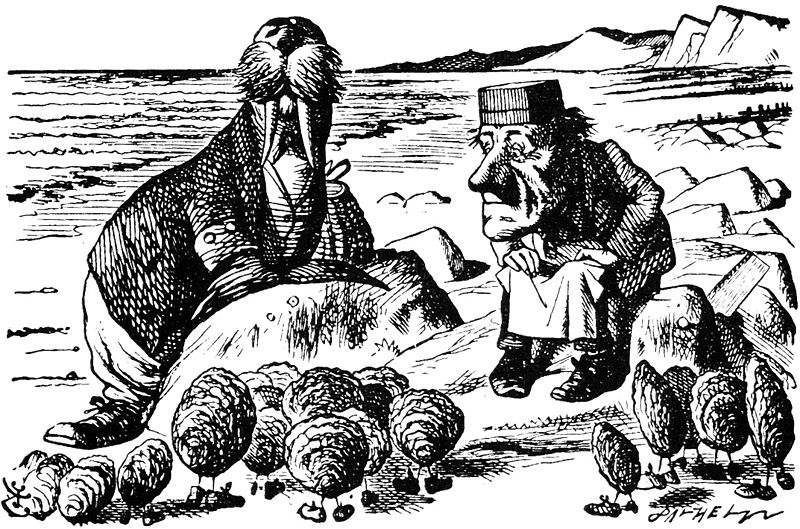
\includegraphics{800px-Briny_Beach.jpg}
\end{center}
\caption[Poem]{The Walrus and the Carpenter}
\label{fig:walrus}
\end{figure}

\section{การเตรียมข้อมูล (Data Preparation)}
\subsection{การโหลดและอ่านชุดข้อมูล (Data Loading)}
\hspace{2em} ขั้นตอนแรกคือการนำเข้าชุดข้อมูลที่ใช้สำหรับการทดลอง SWaT Dataset ซึ่งเป็นข้อมูลการทำงานของระบบน้ำในอุตสาหกรรมที่บันทึกค่า sensor และ actuator ในรูปแบบ time-series 
การโหลดข้อมูลอาจใช้เครื่องมืออย่าง Pandas เพื่ออ่านไฟล์ .csv แล้วจัดเก็บให้อยู่ในรูปแบบ DataFrame เพื่อให้สามารถจัดการได้สะดวกในขั้นตอนถัดไป

\subsection{การจัดการค่าที่หายไป (Missing Value Handling)}
\hspace{2em} ข้อมูลที่ได้จากระบบ OT/ICS มักมีปัญหาค่าที่หายไป (missing values) อันเนื่องมาจากปัญหาของ sensor หรือการบันทึกข้อมูล การจัดการอาจทำได้หลายวิธี เช่น
\begin{enumerate}
  \item การลบข้อมูลแถวที่หายไป (listwise deletion)
  \item การแทนค่าด้วยสถิติพื้นฐาน (เช่น ค่าเฉลี่ย ค่ามัธยฐาน)
  \item การแทนค่าด้วยการคำนวณจากข้อมูลรอบข้าง เช่น interpolation ในกรณีข้อมูลเชิงเวลา
\end{enumerate}

\subsection{การแยกประเภทคุณลักษณะ (Continuous / Discrete Features)}
\hspace{2em} ชุดข้อมูลมักประกอบด้วยคุณลักษณะหลายประเภท เช่น
\begin{enumerate}
  \item Continuous features: ค่าเซนเซอร์ เช่น ความดัน, อัตราการไหล
  \item Discrete features: ค่าสถานะ actuator เช่น เปิด/ปิดวาล์ว, เปิด/ปิดปั๊ม \\ การแยกประเภทคุณลักษณะมีความสำคัญเพราะวิธี preprocessing อาจแตกต่างกัน เช่น continuous ต้อง scaling แต่ discrete อาจใช้ encoding
\end{enumerate}

\subsection{การปรับสเกลข้อมูล (Scaling and Normalization)}
\hspace{2em} ค่าของเซนเซอร์บางตัวอาจอยู่ในช่วงที่ต่างกันมาก เช่น อุณหภูมิ (0–100) กับค่าแรงดัน (0–10,000) หากไม่ปรับสเกล อาจทำให้โมเดลให้ความสำคัญกับตัวแปรที่มีค่ามากเกินไป โดยใช้วิธี
\begin{center}
  Min-Max Scaling (ปรับให้อยู่ในช่วง [0,1])
\end{center}

\subsection{การแบ่งชุดข้อมูล (Training / Testing Split)}
\hspace{2em} เพื่อป้องกันการ overfitting ต้องแบ่งข้อมูลออกเป็น training set และ testing set เช่น 70/30 หรือ 80/20 ในงาน time-series อาจต้องใช้ sliding window ในการแบ่ง โดยไม่ทำการ shuffle ข้อมูล เพื่อคงลำดับเวลาให้ถูกต้อง

\section{การทำ Feature Engineering}

\subsection{การเลือกคุณลักษณะที่เกี่ยวข้อง (Feature Selection)}
\hspace{2em} ไม่ใช่ทุกคุณลักษณะมีความสำคัญต่อการตรวจจับ anomaly การใช้ feature selection จะช่วยลดมิติของข้อมูลและปรับปรุงประสิทธิภาพโมเดล เทคนิคที่ใช้เช่น
\begin{enumerate}
  \item การวิเคราะห์ Correlation Matrix
  \item การใช้ Mutual Information
  \item การใช้ Model-based feature selection เช่น Random Forest
\end{enumerate}


\subsection{การใช้ Sliding Window กับ Time-series Data}
\hspace{2em} เนื่องจากข้อมูล ICS/OT เป็น time-series จำเป็นต้องแปลงข้อมูลให้อยู่ในรูป window-based input เช่น สร้าง sequence ขนาด 30 หรือ 60 วินาที เพื่อใช้ในการเรียนรู้ pattern ของระบบ วิธีนี้ช่วยให้โมเดล CNN/LSTM สามารถตรวจจับลักษณะของ anomaly ที่เกิดขึ้นในช่วงเวลาได้

\subsection{การสร้างคุณลักษณะใหม่ (Derived Features)}
\hspace{2em} สามารถสร้าง feature เพิ่มเติมจากข้อมูลดิบ เช่น
\begin{enumerate}
  \item ค่า moving average ของเซนเซอร์
  \item ค่าความแตกต่างระหว่างเวลา ($\Delta t$)
  \item อัตราการเปลี่ยนแปลง (derivatives) \\ สิ่งเหล่านี้ช่วยให้โมเดลจับความผิดปกติได้ดีกว่าการใช้ข้อมูลดิบเพียงอย่างเดียว
\end{enumerate}

\subsection{การตรวจสอบความสัมพันธ์ของคุณลักษณะ (Correlation Analysis)}
\hspace{2em} การวิเคราะห์ความสัมพันธ์ระหว่าง features เช่น การคำนวณ Pearson Correlation หรือ Spearman Rank Correlation เพื่อดูว่าคุณลักษณะใดสัมพันธ์กันมากเกินไป หาก correlation สูง อาจเลือกตัดบาง feature ทิ้งเพื่อลด redundancy

\section{การออกแบบและพัฒนาโมเดล (Model Design and Development)}

\subsection{การเลือกโมเดลต้นแบบ (CNN Prototype)}
\hspace{2em} เลือกใช้ Convolutional Neural Network (CNN) เพราะสามารถจับ pattern ในข้อมูล time-series ได้คล้ายกับการประมวลผลภาพ โดยมองว่าแต่ละ sequence เป็น “สัญญาณหลายมิติ” จาก sensor และ actuator

\subsection{สถาปัตยกรรมของโมเดล (Model Architecture)}
\hspace{2em} Input Layer: รับข้อมูล time-series ที่ผ่าน preprocessing แล้ว
\begin{enumerate}
  \item Input Layer: รับข้อมูล time-series ที่ผ่าน preprocessing แล้ว
  \item Convolutional Layer: ดึง pattern ที่ซ่อนอยู่จากข้อมูล เช่น ความเปลี่ยนแปลงของ sensor
  \item Pooling Layer: ลดมิติและ noise ทำให้โมเดล generalize ได้ดีขึ้น
  \item Fully Connected Layer: รวม feature ที่สกัดมาเพื่อใช้ในการจำแนก anomaly
  \item Output Layer: ใช้ softmax/sigmoid เพื่อตัดสินว่าเป็น “ปกติ” หรือ “ผิดปกติ”
\end{enumerate}

\subsection{การตั้งค่า Hyperparameters}
\hspace{2em} กำหนดค่าเช่น learning rate, batch size, จำนวน epoch, จำนวน filter และ kernel size ใน CNN การเลือกค่าเหล่านี้มีผลโดยตรงต่อความแม่นยำและความเร็วของการเรียนรู้

\subsection{เครื่องมือและ Framework ที่ใช้ (เช่น TensorFlow / PyTorch)}
\hspace{2em} เช่น TensorFlow, PyTorch, Scikit-learn ใช้ร่วมกับ Google Colab (GPU) เพื่อประมวลผลได้เร็วขึ้น

\section{การทดสอบและประเมินผล (Experiment and Evaluation)}

\subsection{วิธีการแบ่งชุดข้อมูลสำหรับทดสอบ (Train/Test Strategy)}
\hspace{2em} ใช้ hold-out method (train/test split) หรือ cross-validation สำหรับ time-series อาจใช้ walk-forward validation เพื่อเลียนแบบสถานการณ์จริง

\subsection{ตัวชี้วัดประสิทธิภาพ (Evaluation Metrics)}
\begin{enumerate}
  \item Accuracy: วัดความถูกต้องโดยรวม
  \item Precision, Recall, F1-score: วัดความสามารถในการตรวจจับ anomaly โดยไม่แจ้งเตือนผิดพลาด
  \item Detection Rate (DR), False Alarm Rate (FAR): เน้นการประเมินประสิทธิภาพในการตรวจจับโจมตีและลด false positive
\end{enumerate}

\section{การประยุกต์ใช้งานและข้อจำกัด (Application and Limitations)}
\subsection{ศักยภาพในการนำไปใช้จริง (Practical Applications)}
\hspace{2em} ระบบที่พัฒนาสามารถนำไปใช้ใน โรงงานอุตสาหกรรม เพื่อช่วยตรวจจับพฤติกรรมผิดปกติของเซนเซอร์หรือ อุปกรณ์ เช่น การโจมตีปั๊มน้ำ หรือการเปิดวาล์วโดยไม่ได้รับอนุญาต

\subsection{ข้อจำกัดของโครงงาน (Limitations)}
\begin{enumerate}
  \item ใช้ข้อมูลจำลอง (SWaT dataset) แทนข้อมูลจริง
  \item ทดสอบในสภาพแวดล้อมจำกัด ไม่ครอบคลุมทุกประเภทของการโจมตี
  \item ความแม่นยำอาจลดลงหากนำไปใช้กับ dataset อื่นที่มีลักษณะแตกต่าง
\end{enumerate}

\subsection{แนวทางการพัฒนาในอนาคต (Future Work)}
\begin{enumerate}
  \item ทดลองใช้โมเดล Hybrid (CNN+LSTM)
  \item นำ model ไปใช้ในการทำระบบเตือน โดยผ่าน API หรือ Websocket
\end{enumerate}
\chapter{\ifproject%
\ifenglish Experimentation and Results\else การทดลองและผลลัพธ์\fi
\else%
\ifenglish System Evaluation\else การประเมินระบบ\fi
\fi}

\section{วัตถุประสงค์การทดสอบ (Objective)}
\hspace{2em} การประเมินผลของโครงงานนี้มีจุดประสงค์เพื่อวิเคราะห์ประสิทธิภาพของโมเดล CNN-LSTM \\ ที่พัฒนาขึ้นสำหรับการตรวจจับความผิดปกติ (Anomaly Detection) ใน SWaT dataset โดยมีวัตถุประสงค์สำคัญดังนี้:
\begin{enumerate}
    \item ตรวจสอบความสามารถของโมเดลในการจำแนกสถานะ ปกติ (Normal) และ ผิดปกติ (Anomaly) จากข้อมูล time-series ของ sensor และ actuator
    \item ประเมินประสิทธิภาพตามตัวชี้วัดมาตรฐาน ได้แก่ Precision, Recall, F1-score, Area Under Curve (ROC-AUC, PR-AUC) เพื่อวัดความแม่นยำเชิงสถิติ
    \item วิเคราะห์ Detection Delay และ Latency เพื่อพิจารณาความเหมาะสมในการใช้งานเชิงปฏิบัติการแบบ real-time
    \item ทดสอบความทนทาน (Robustness) ของโมเดลต่อเงื่อนไขที่อาจเกิดขึ้นจริง เช่น
    \begin{itemize}
        \item Noise จากความผันผวนของ sensor
        \item Missing data (ข้อมูลสูญหายระหว่างการเก็บ)
        \item Concept drift หรือ pattern ใหม่ที่ไม่เคยปรากฏมาก่อน
    \end{itemize}
    \item เปรียบเทียบผลลัพธ์กับโมเดล baseline เช่น CNN เดี่ยว, LSTM เดี่ยว, Autoencoder เพื่อยืนยันความเหมาะสมของ CNN-LSTM
\end{enumerate}

\section{Requirements (ข้อกำหนดการทดสอบ)}
\subsection{Functional Requirements (ข้อกำหนดเชิงฟังก์ชัน)}
\begin{enumerate}
    \item โมเดลต้องสามารถจำแนกข้อมูล Normal vs Anomaly ได้อย่างถูกต้อง
    \item ระบบต้องสามารถ แจ้งเตือน (Alert System) ได้ทั้งแบบ batch processing และ real-time detection
    \item รองรับการนำเข้าข้อมูลจาก sensor/actuator ที่มีโครงสร้างตาม SWaT dataset
    \item มีการจัดเก็บและนำเสนอผลลัพธ์ในรูปแบบ visualization และ log files (เช่น confusion matrix, error curves)
\end{enumerate}

\subsection{Non-Functional Requirements (ข้อกำหนดไม่เชิงฟังก์ชัน)}
\begin{enumerate}
    \item Accuracy Benchmark: ค่าคะแนน F1-score ต้องไม่ต่ำกว่า $\ge$ 85\% (อ้างอิง benchmark งานวิจัยที่เกี่ยวข้อง)
    \item Latency: การทำนายผลแต่ละ window ต้องใช้เวลา ≤ 20 ms เพื่อรองรับ real-time operation
    \item Robustness: ประสิทธิภาพต้องลดลงไม่เกิน $\ge$ 10\% ภายใต้เงื่อนไข noise หรือ missing data
    \item Scalability: รองรับจำนวน sensor อย่างน้อย 50 ตัว และ batch size ≥ 64
    \item Usability: ผลลัพธ์ต้องสามารถแสดงในรูป ตารางและกราฟ ที่เข้าใจง่ายต่อผู้ปฏิบัติการ
\end{enumerate}

\subsection{Dataset Requirements}
\begin{enumerate}
    \item ใช้ SWaT dataset โดยแบ่งเป็น Normal logs สำหรับการฝึกโมเดล และ Normal + Attack logs สำหรับการทดสอบ
    \item การแบ่งข้อมูลต้องเป็น Training / Validation / Testing sets โดยพิจารณาลำดับเวลาเพื่อป้องกัน data leakage
    \item ต้องทำการ Preprocessing เช่น normalization, sliding window, และการแทนค่าข้อมูลที่หายไป (imputation)
\end{enumerate}

\section{กลยุทธ์การทดสอบ (Testing Strategy)}
\subsection{ประเภทของการทดสอบ (Types of Testing)}
\begin{enumerate}
    \item Functional Testing
    \begin{enumerate}
        \item ตรวจสอบความถูกต้องในการจำแนก anomaly ใน test set
        \item ทดสอบการทำงานของ alert system ในสภาพ online detection
    \end{enumerate}
    \item Performance Testing
    \begin{enumerate}
        \item ประเมินผลด้วย Precision, Recall, F1-score, ROC-AUC และ PR-AUC
        \item วัด latency และ throughput ของระบบ
    \end{enumerate}
    \item Robustness Testing
    \begin{enumerate}
        \item เพิ่ม noise ลงในข้อมูล sensor และวัดผลลัพธ์
        \item จำลองการ missing values แบบสุ่มและวิเคราะห์ผลกระทบ
        \item ทดสอบ response ต่อ concept drift หรือการโจมตีที่ไม่เคยปรากฏใน training
    \end{enumerate}
    \item Comparison Testing
    \begin{itemize}
        \item เปรียบเทียบกับ baseline models ได้แก่ LSTM, CNN, Autoencoder
        \item วิเคราะห์ผลลัพธ์เพื่อยืนยันข้อดีของโมเดล CNN-LSTM
    \end{itemize}
\end{enumerate}
%\ifproject
%\include{chapters/conclusion}
%\fi

\bibliography{myReport}

% \ifproject
% \normalspacing
% \appendix
% \include{chapters/appendix}

%% Display glossary (optional) -- need glossary option.
\ifglossary\glossarypage\fi

%% Display index (optional) -- need idx option.
\ifindex\indexpage\fi

% \begin{biosketch}
% \begin{center}
%   \includegraphics[width=1.5in]{mugshot.jpg}
% \end{center}
% Your biosketch goes here. Make sure it sits inside
% the \texttt{biosketch} environment.
% \end{biosketch}
% \fi % \ifproject
\end{document}
